\documentclass[a4paper]{article}
\usepackage{graphicx}
\usepackage{amsmath, amsfonts, geometry, float, listings, enumerate, multicol}
\usepackage{multicol, float, color, colortbl}
\usepackage{tikz, titlesec, parskip, pgfplots, filecontents}
\usepackage{hyperref}
\usepackage{amsmath}
\usepackage{tikz, titlesec, parskip}
\usepackage{tikz,pgfplots}
\usepackage[americanvoltages,fulldiodes,siunitx]{circuitikz}
\usetikzlibrary{shapes,arrows}
\usepackage{enumitem}
\titleformat*{\subsubsection}{\LARGE\bfseries}

\titlespacing{\section}{0pt}{10pt}{0pt}
\titlespacing{\subsection}{0pt}{10pt}{0pt}
\titlespacing{\subsubsection}{0pt}{10pt}{0pt}



\usetikzlibrary{calc,patterns,through}
\newcommand{\arcangle}{%
	\mathord{<\mspace{-9mu}\mathrel{)}\mspace{2mu}}%
}

\renewcommand{\baselinestretch}{1.4}
 \geometry{
 a4paper,
 total={170mm,257mm},
 left=20mm,
 top=20mm,
 }
\usepackage{fancyhdr}
\usepackage{indentfirst}
\pagestyle{fancy}
\fancyhf{}
\rhead{\textbf{پردازش تصاویر دیجیتال}}
\lhead{\textbf{تمرین سری اول}}
\cfoot{(\space \space \space \space \textbf{\thepage}  \space \space \space)}
\renewcommand{\headrulewidth}{1pt}
\renewcommand{\footrulewidth}{1pt}

 
\usepackage{xepersian}
\setlatintextfont{Times New Roman}
\settextfont{XB Niloofar}
\setdigitfont{XB Niloofar}
\DefaultMathsDigits

\makeatletter
\bidi@patchcmd{\@Abjad}{آ}{الف}
{\typeout{Succeeded in changing آ into الف}}
{\typeout{Failed in changing آ into الف}}
\makeatother
\PersianAlphs

\begin{document}
\begin{minipage}{0.6\textwidth}
\begin{bf}
\begin{center}
	به نام خدا\\
	\vspace{0.25cm}
	دانشگاه صنعتی شریف\\
	\vspace{0.25cm}
	دانشکده مهندسی برق\\
	\vspace{0.5cm}

\large
دکتر عمادالدین فاطمی‌زاده - پردازش تصاویر دیجیتال \\
نیم سال دوم
۱۴۰۱-۱۴۰۰\\
\Large
\vspace{0.4cm}
تمرین عملی سری اول\\
\end{center}
\end{bf}
\normalsize
\end{minipage} \hfill
\begin{minipage}{0.35\textwidth}
\begin{flushleft}

\includegraphics[width=0.5\textwidth]{Shariflogo.png}\\ \large
\end{flushleft}

 \end{minipage}
\\

\rule[0.1\baselineskip]{\textwidth}{1pt}

\large
\section*{
لطفاً به نکات زیر توجه بفرمایید: (رعایت نکردن این موارد باعث کاهش نمره می‌شود.)
}

\begin{enumerate}
	\item 
نتایج و پاسخ های خود را در یک فایل با فرمت zip به نام
\LR{HW$1$-Name-StudentNumber}
 در سایت  
\href{https://quera.org/course/add_to_course/course/10598/}{\lr{Quera}} 
 قرار دهید. همچنین فایل پایتون یا متلب خود را به همان نام در قسمت مخصوص به خود آپلود کنید.
\item 
کسب نمره کامل در هر سوال مستلزم تحویل  
\textbf{کدها (40 نمره)}
 و
\textbf{توضیحات (30 نمره)}
و
\textbf{نتایج (30 نمره)}
 می‌باشد. 
\item 
کدهای شما تماماً باید توسط خودتان نوشته شده باشند. هرگونه استفاده از کد دیگران، اعم از دوستان و اینترنت، به هر شکل ممکن، تقلب محسوب می‌شود و نمره تمام تمرینات جاری و تمام تمرینات قبلی صفر خواهد شد. با اجرای این کدها باید همان نتایجی که فرستاده اید قابل بازیابی باشند. برنامه شما باید به گونه ای باشد که بدون نیاز به هیچ تغییری قابل اجرا باشد، در غیر اینصوررت هیچ نمره ای تعلق نخواهد گرفت. 
\item 
برای تمام سؤالات، باید جزئیات روشی که استفاده کرده‌اید را توضیح دهید و نتایجی که گرفته‌اید را ارائه دهید. این توضیحات می‌تواند در یک فایل  pdf  و یا در یک فایل  ipynb باشد. در توضیحات، باید اشاره کامل به کارهایی که انجام داده‌اید بنمایید به طوری که یک شخص آگاه از موارد درس بتواند به آسانی متوجه کاری که شما انجام داده‌اید شود.
\item 
در طول ترم امکان ارسال با تاخیر پاسخ  همه‌ی تمارین تا سقف پنج روز و در مجموع بیست و یک روز وجود دارد. پس از گذشت این مدت، پاسخ‌های ارسال‌شده پذیرفته نخواهند بود. همچنین، به ازای هر روز تأخیر غیر مجاز  بیست درصد از نمره تمرین به صورت ساعتی کسر خواهد شد.
\item 
مهلت تحویل: 18 اسفند ساعت 23:59 
\item 
نام طراح هر سوال در زیر آن نوشته شده است و شما میتوانید سوالات خود را از طریق ایمیل یا تلگرام از طراح سوال بپرسید.
\\
یاسمین مدقالچی: 
 \href{mailto:Yasmed1379@yahoo.com}{Yasmed1379@yahoo.com}
 - 
 \lr{@Yasssssimed}
\\
صدرا صبوری: 
 \href{mailto:Sadra@ee.sharif.edu}{Sadra@ee.sharif.edu}
 - 
 \lr{@Sadrasabouri}
\end{enumerate}
\rule[0.1\baselineskip]{\textwidth}{1pt}

\clearpage
\textbf{\huge
	تمارین تئوری
}

\vspace{0.5cm}
\textbf{\LARGE
	سوال اول
}
\\
\textbf{طراح :‌ صدرا صبوری}
\\
در تبدیلات هندسی خطی گاهی اوقات ممکن است تصویر تبدیل‌شده به درستی در فضای مقصد جای نگیرد و بعضی از پیکسل ها بدون مقدار رها شوند 
(شکل 
\ref{Inverse Warping}
).
برای جلوگیری از این اتفاق از تکنیک جالبی (برای اطلاعات بیشتر به  
\href{https://www.researchgate.net/publication/267946997_Non-rigid_Registration_Using_Free-form_Deformations}{اینجا}
مراجعه کنید) استفاده می‌شود. با توجه به اینکه تبدیل خطی است، پس وارون‌پذیر هم هست. حال کافی است اندیس متناظر با هر پیکسل از فضای مقصد را با اعمال تبدیل خطی معکوس روی آن، به فضای مبدا بیاوریم.
\begin{figure}[H]
	\centering
	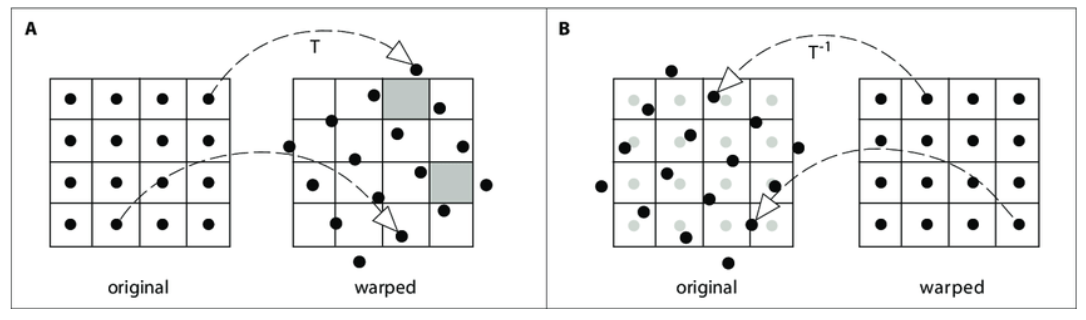
\includegraphics[width=0.8 \linewidth]{images/Q5_1.png}
	\caption{\lr{Forward Warping and Inverse Warping}}
	\label{Inverse Warping}
\end{figure}

همانطور که در شکل
\ref{Interpolation} 
میبینید بعد از این تبدیل تعدادی از نقاط به صورت دقیق روی پیکسل خاصی قرار نگرفته‌اند. به عنوان مثال فرض کنید مختصات فضای مبدا مورد نظر در $ (x+a, y+b)  $ قرار گرفته‌است. پیشنهاد شما برای انتخاب مقدار پیکسل فضای مقصد با توجه به مقادیر زیر چه مقداری است؟ (راهنمایی: بهتر است جواب به گونه‌ای باشد که با نزدیک شدن به یکی از $ 4 $ پیکسل اصلی فضای مبدا مقدار نهایی پیکسل به مقدار آن پیکسل میل کند.)

\begin{figure}[h]
	\centering
	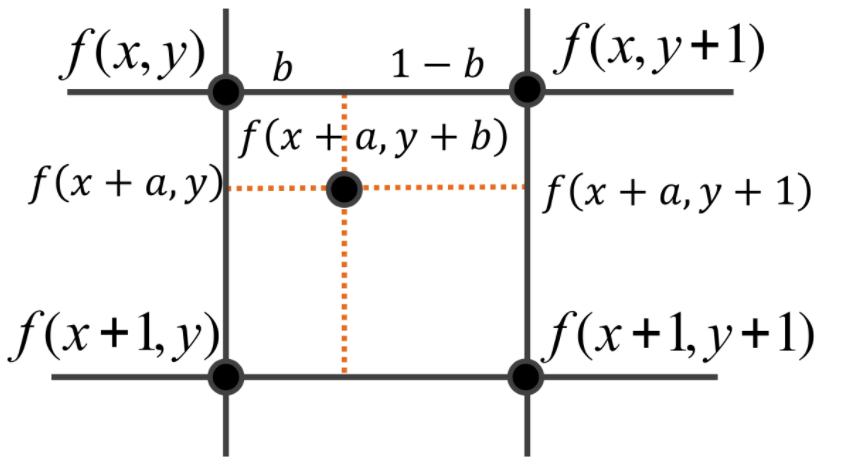
\includegraphics[width=0.45 \linewidth]{images/Q5_2.png}
	\caption{\lr{Interpolation}}
	\label{Interpolation}
\end{figure}

\textbf{\LARGE
	سوال دوم
}
\\
\textbf{طراح :‌ صدرا صبوری}
\\
جدول زیر محتویات تصویری است که می‌خواهیم آن را در جهت افقی و عمودی بزرگ کنیم.
 \begin{figure}[H]
	\centering
	\begin{tabular}{ | c | c | c | }
		\hline			
		\lr{106} & \lr{110} & \lr{107} \\
		\hline	
		\lr{104} & \lr{105} & \lr{106} \\
		\hline	
		\lr{140} & \lr{142} & \lr{138} \\
		\hline  
	\end{tabular}
\end{figure}
زمانی که تصویر را بزرگ می‌کنیم مقادیر تعدادی از خانه‌ها که در تصویر ابتدایی نبودند را می‌بایست به کمک درون‌یابی مقداردهی کنیم. جدول زیر که نمایش تصویر بزرگ‌شده است را کامل کنید و روش درون‌یابی خود را توضیح دهید.
 \begin{figure}[H]
	\centering
	\begin{tabular}{ | c | c | c | c | c |}
		\hline			
		\lr{106} & $\;\;\;$ & \lr{110}  & $\;\;\;$ & \lr{107} \\
		\hline	
		$\;\;\;$ & $\;\;\;$ & $\;\;\;$  & $\;\;\;$ & $\;\;\;$ \\
		\hline
		\lr{104} &  $\;\;\;$ & \lr{105} &$\;\;\;$ & \lr{106} \\
		\hline	
		$\;\;\;$ & $\;\;\;$ & $\;\;\;$  & $\;\;\;$ & $\;\;\;$ \\
		\hline
		\lr{140} &$\;\;\;$ & \lr{142} &  $\;\;\;$ & \lr{138} \\
		\hline  
	\end{tabular}
\end{figure}
\textbf{\LARGE
	سوال سوم
}
\\
\textbf{طراح :‌ صدرا صبوری}
\\
ادعا می‌شود که رنگ دو خانه A و B شکل 
\ref{House Image}
با هم یکسان است. سعی کنید خانه A و B را جدا کنید و با نام 
\lr{House\_A}
و
\lr{House\_B}
ذخیره کنید. این دو تصویر را با هم مقایسه کنید.
\begin{figure}[h]
	\centering
	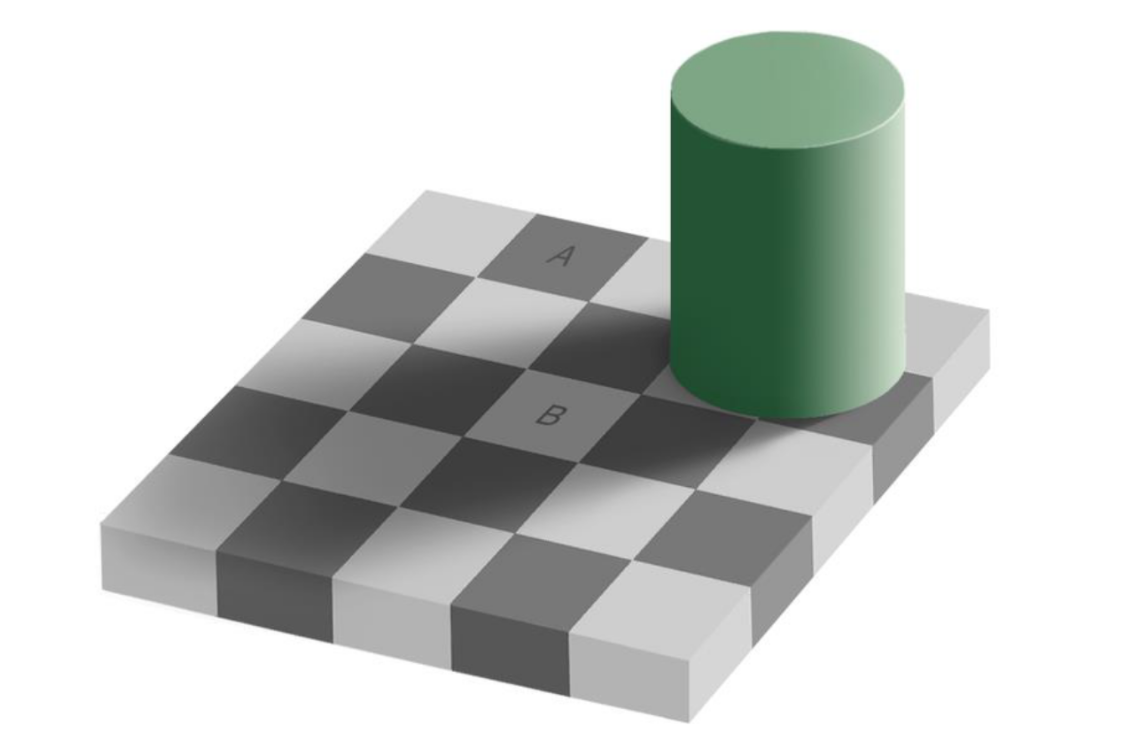
\includegraphics[width=0.5\linewidth]{images/Q2_1.png}
	\caption{ \lr{Checker shadow illusion}}
	\label{House Image}
\end{figure}


\rule[0.1\baselineskip]{\textwidth}{1pt}

\textbf{\huge
تمارین عملی
}

\vspace{0.5cm}
\textbf{\LARGE
	سوال اول
}
\\
\textbf{طراح :‌ یاسمین مدقالچی}
\begin{enumerate}
	\item 
عکس 
\lr{campusdrive.png}
را بخوانید. ابتدا مشخص کنید که ساختار عکس چند بیتی است؟
\item
در یک حلقه تعداد بیت quantization آن را کاهش دهید و نتیجه را به صورت چند عکس نمایش دهید. کیفیت عکس تا چه مرحله‌ای قابل قبول می‌ماند ؟
	\item 
حال درون حلقه برای هر
 \lr{quantization bit}
 چند ماسک رندوم تولید کنید. این ماسک ماتریسی به ابعاد تصویر است که هر خانه‌ی آن به صورت رندوم از $ 0 $ یا $ 1 $ پر شده‌است. می‌خواهیم  تنها تغییر بیت
 \lr{quantization}
 روی پیکسل‌هایی اعمال شود که مقدار آن پیکسل در ماسک تولید شده $ 1 $ باشد و بقیه پیکسل‌ها دست نخورده باقی بمانند. نتیجه ماسک‌های مختلف بر روی 
\lr{quantization bit}
های مختلف را به صورت پشت سر هم به صورت گیف نمایش دهید و با نام 
\lr{quantized\_campusdrive}
ذخیره کنید.
\end{enumerate}
\newpage
\textbf{\LARGE
سوال دوم
}
\\
\textbf{طراح :‌ صدرا صبوری}
\\
فایل 
\lr{SharifLogo}
 را بخوانید. حجم تصویر را با کمک ابعاد تصویر و تعداد بیت مورد استفاده در هر پیکسل به دست بیاورید. چرا حجم بدست آمده با حجم واقعی تصویر متفاوت است؟ درصد فشرده‌سازی را به دست بیاورید.

\textbf{\LARGE
	سوال سوم
}
\\
\textbf{طراح :‌ صدرا صبوری}
\\
در این سوال قصد داریم از تکنیک‌های 
\lr{Image Enhancement}
 استفاده کنیم و در آخر یک gif مشابه شکل 
 \ref{Traumatized Mr.Incredible}
 بسازیم
 \RTLfootnote{
 	برای آشنایی بیشتر عبارت
 	\lr{Traumatized Mr.Incredible} 
 	را جست و جو کنید.
 }.
\begin{figure}[H]
	\centering
	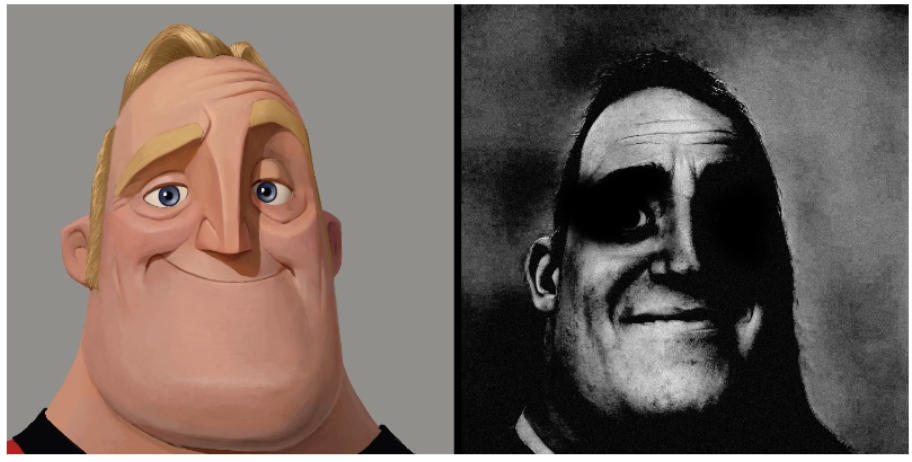
\includegraphics[width=0.5 \linewidth]{images/Q6_1.png}
	\caption{\lr{Traumatized Mr.Incredible}}
	\label{Traumatized Mr.Incredible}
\end{figure}  
\begin{enumerate}
	\item 
تصویر 
\lr{bigMasoud.jpg}
 را بخوانید و به آرامی شروع به تاریک کردن تصویر کنید. 
  به ازای هر میزان روشنایی، یک تصویر ذخیره کنید. دقت کنید که روند تاریک شدن تصویر در همه جای تصویر به شکل یکنواخت نیست. سعی کنید با استفاده از روش‌های خلاقانه کیفیت عکس‌ها و خروجی نهایی را افزایش دهید. در آخر با به هم چسباندن این تصاویر یک فایل 
 \lr{gif} 
 یا ویدیو تولید کنید و با نام 
 \lr{Traumatized\_bigMasoud}
 ذخیره کنید.
 \item
دو تصویر از این مجموعه تصاویر (که تفاوت روشنایی آن‌ها با یکدیگر معنی‌دار است) را انتخاب کنید و هیستوگرام سه کانال رنگی آن‌ها را به عنوان خروجی نمایش دهید و با نام‌های 
\lr{Histogram\_Img1}
و 
\lr{Histogram\_Img2}
ذخیره کنید.
\end{enumerate}
\end{document}
